
%%%%%%%%%%%%%%%%%%%%%%%%%%%%%%%%%%%%%%%%%%%%%%%%%%%%%%%%%%%%%%%%%%%%%%%%%%%%%
%%%%% Traversing a mesh %%%%%%%%%%%%%%%%%%%%%%%%%%%%%%%%%%%%%%%%%%%%%%%%%%%%%
%%%%%%%%%%%%%%%%%%%%%%%%%%%%%%%%%%%%%%%%%%%%%%%%%%%%%%%%%%%%%%%%%%%%%%%%%%%%%
\begin{frame}
\pointedsl{
	Exploration
}
\end{frame}

% TODO
% Content:
% 1. Iterators (vertex, edges, half-edges, faces)
% 2. Manual: looping over the boundary
% 3. Manual: 1-ring vertex traversal
% 4. Circulators (vertex, edges, half-edges, faces)

%%%%%%%%%%%%%%%%%%%%%%%%%%%%%%%%%%%%%%%%%%%%%%%%%%%%%%%%%%%%%%%%%%%%%%%%%%%%%
\begin{frame}[fragile]
\frametitle{Iterators}
\misc{
	\textbf{Iterators} are used to traverse all the elements of a specific type (\emph{vertices}, \emph{halfedges}, \emph{edges} or \emph{faces}).
}
\begin{lstlisting}
// iterating over all vertices
Surface_mesh::Vertex_iterator vit, vend;
for(vit = mesh.vertices_begin(),
    vend = mesh.vertices_end();
    vit != vend; ++vit){
  Vertex v = *vit;
  // do something with vertex v
}
\end{lstlisting}
\end{frame}

\begin{frame}[fragile]
\frametitle{Iterators}
\begin{lstlisting}
// iterating over all XXX
Surface_mesh::Halfedge_iterator hit;
hit = mesh.halfedges_begin();

Surface_mesh::Edge_iterator eit;
eit = mesh.edges_begin();

Surface_mesh::Face_iterator fit;
fit = mesh.faces_begin();
\end{lstlisting}
\misc{
	Iterators traverse elements in the order they are stored in memory.
	\textbf{You should not expect any ordering.}
}
\end{frame}

%%%%%%%%%%%%%%%%%%%%%%%%%%%%%%%%%%%%%%%%%%%%%%%%%%%%%%%%%%%%%%%%%%%%%%%%%%%%%
\begin{frame}
\framedsl{
	Iterating regions?
}
\end{frame}

\begin{frame}
\frametitle{The boundary -vs- inside}
\begin{center}
	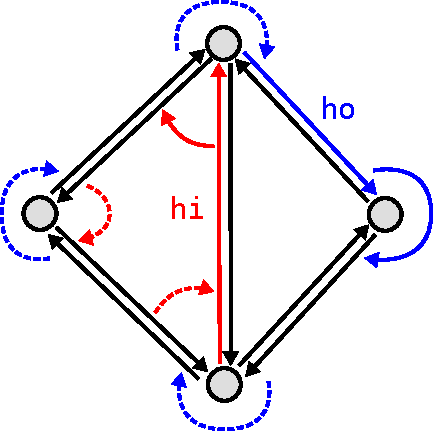
\includegraphics[width=0.42\textwidth]{figures/halfedges-boundaries}
\end{center}
\misc{
	Using half-edge connectivity, it is easy to traverse a face.
	
	If a half-edge is on the boundary side (it has no face linked to it),
	then this results in going over the whole boundary.
}
\end{frame}

\begin{frame}[fragile]
\frametitle{The boundary -vs- inside}
\begin{lstlisting}
Surface_mesh::Halfedge ho, h;

// traversing the boundary
h = ho;
do {
  // use h
  h = mesh.next_halfedge(h);
} while(h != ho);
\end{lstlisting}
\misc{
	Replace \ctext{ho} by \ctext{hi} to traverse the half-edges of a face.
}
\end{frame}

%%%%%%%%%%%%%%%%%%%%%%%%%%%%%%%%%%%%%%%%%%%%%%%%%%%%%%%%%%%%%%%%%%%%%%%%%%%%%
\begin{frame}
\frametitle{Vertex 1-ring}
\begin{center}
	\includegraphics[width=0.42\textwidth]{figures/vertex-1ring}
\end{center}
\misc{
	Using half-edge connectivity, it is easy to traverse the \textbf{1-ring} neighborhood
	of a vertex \ctext{c}.
}
\end{frame}

\begin{frame}[fragile]
\frametitle{Vertex 1-ring}
\begin{lstlisting}
Surface_mesh::Vertex c, v;
Surface_mesh::Halfedge h, h0;

// traversing the 1-ring
h = h0 = mesh.halfedge(c);
do {
  // get vertex
  v = mesh.to_vertex(h);
  // get next half-edge
  h = mesh.opposite_halfedge(h);
  h = mesh.next_halfedge(h);
} while(h != ho);
\end{lstlisting}
\end{frame}

%%%%%%%%%%%%%%%%%%%%%%%%%%%%%%%%%%%%%%%%%%%%%%%%%%%%%%%%%%%%%%%%%%%%%%%%%%%%%
\begin{frame}
\frametitle{Circulators}
\misc{
	These kinds of local region iterations are so common that there are a special kind of iterators called \textbf{circulators} which take care of such operations:
	\begin{itemize}
		\item \ctext{Vertex\_around\_vertex\_circulator}
		\item \ctext{Halfedge\_around\_vertex\_circulator}
		\item \ctext{Face\_around\_vertex\_circulator}
		\item \ctext{Vertex\_around\_face\_circulator}
		\item \ctext{Halfedge\_around\_face\_circulator}
	\end{itemize}
}
\end{frame}

\begin{frame}[fragile]
\frametitle{Vertex 1-ring}
\begin{lstlisting}
typedef Surface_mesh Mesh;
Mesh::Vertex c, v;
Mesh::Vertex_around_vertex_circulator 
    vit, vit_end;

vit = vit_end = mesh.vertices(c);
do {
  v = *vit;
  // use 1-ring vertex
} while(++vit != vit_end);

// similarly with
// - mesh.halfedges(v);
// - mesh.faces(v);
// - mesh.vertices(f);
// - mesh.halfedges(f);
\end{lstlisting}
\end{frame}
